%%%%%%%%%%%%%%%%%%%%%%%%
% Python 
%%%%%%%%%%%%%%%%%%%%%%%%

\subsubsection{Purpose}
\noindent \ac{EMTG} depends on the Python interpreter and several packages to execute the PyEMTG \ac{GUI} and other PyEMTG utilities. PyEMTG is known to be compatible with \hl{Python 3.7}.\footnote{PyEMTG is known to specifically \emph{not} be compatible with Python 3.10 because wxWidgets is not compatible with Python 3.10.} Therefore, it is strongly recommended that a Python 3.7 environment be created for PyEMTG. There are multiple ways to get Python but we strongly recommend/support Mambaforge/miniforge. The intstructions in this guide will show a user how to install Python, a user with a preexisting Python install and knowledge on using the correct environments can utilize their own Python install.

\subsubsection{Download Location}
\noindent The main page for the software distributions is in the following website: \\
\url{https://github.com/conda-forge/miniforge/}

\noindent The software package needed for the EMTG version indicated in this guide can be obtained from the following location: \\
\emph{(In the event the url is no longer active, navigate to the aforementioned software website to find the specific version)} \\
\url{https://github.com/conda-forge/miniforge/releases/tag/22.9.0-2/}

\noindent Instructions are given for creating an appropriate Python environment using the Mamba package manager. Information on obtaining and using Mamba is available at \url{https://mamba.readthedocs.io/en/latest/#}. 

\subsubsection{Dependency Installation Instructions}
\begin{enumerate}
	\item Download the Mambaforge-22.9.0-2-Windows-x86\_64.exe installer and install locally. \\ \emph{This is the installer with just mamba as the base environment}
	\item During installation, install mambaforge so it is installed just for the user. \\ See the image below for the Windows example of settings to select. 
		\begin{figure}[H]
			\centering
			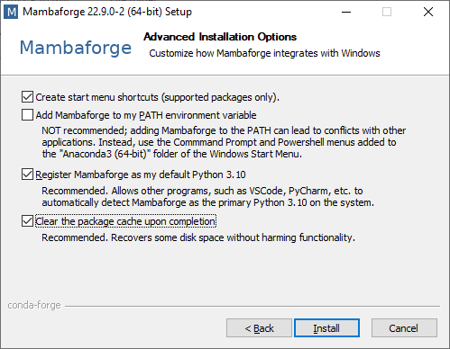
\includegraphics[width=0.5\linewidth]{../../../shared_latex_inputs/images/mambaforge_options.png}
			\caption{Mambaforge Installation Configuration}
		\end{figure}
	\item Open the MiniForge Prompt 
		\begin{figure}[H]
			\centering
			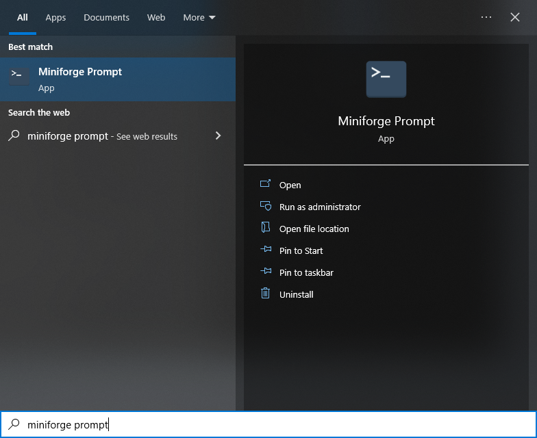
\includegraphics[width=0.5\linewidth]{../../../shared_latex_inputs/images/mambaforge_launch.png}
			\caption{Open Mambaforge Command Prompt}
		\end{figure}
	\item Type the following command and press enter to create the specific python environment for EMTG: \\ 
	\begin{verbatim}
	mamba create -n PyEmtgEnv python=3.7
	\end{verbatim}
	\begin{enumerate}
		\item Accept changes when prompted
	\end{enumerate}
	\item Type the following command and press enter to switch to the new python environment: \\ 
	\begin{verbatim}
		mamba activate PyEmtgEnv
	\end{verbatim}
	\item Enter the following to confirm the python version selected is active: \\
	\begin{verbatim}
		python --version
	\end{verbatim}	
	\item Install the following python packages
	\begin{itemize}
		\item numpy 1.21.6
		\item spiceypy 5.0.1
		\item jplephem 2.17
		\item scipy 1.7.3
		\item matplotlib 3.5.2
		\item wxPython 4.1.1
		\item astropy 4.3.1
		\item pandas 1.3.5
	\end{itemize}
	\begin{enumerate}
		\item The following is the command to use to install the various package versions listed above:\\
		\begin{verbatim}
			pip install packageName==#.#.#
		\end{verbatim}
		\item Here is an example of the command for numpy:
		\begin{verbatim}
			pip install numpy==1.21.6
		\end{verbatim}
	\end{enumerate}
	\item Enter the following to verify the stated versions of the packages were installed: \\
	\begin{verbatim}
		pip list
	\end{verbatim}	
\end{enumerate}
